\documentclass[12pt]{article}
\usepackage[margin=2.5cm]{geometry}
\usepackage{enumerate}
\usepackage{amsfonts}
\usepackage{amsmath}
\usepackage{fancyhdr}
\usepackage{amsmath}
\usepackage{amssymb}
\usepackage{amsthm}
\usepackage{mdframed}
\usepackage{graphicx}
\usepackage{subcaption}
\usepackage{adjustbox}
\usepackage{listings}
\usepackage{xcolor}
\usepackage{booktabs}
\usepackage[utf]{kotex}
\usepackage{hyperref}

\definecolor{codegreen}{rgb}{0,0.6,0}
\definecolor{codegray}{rgb}{0.5,0.5,0.5}
\definecolor{codepurple}{rgb}{0.58,0,0.82}
\definecolor{backcolour}{rgb}{0.95,0.95,0.92}

\lstdefinestyle{mystyle}{
    backgroundcolor=\color{backcolour},
    commentstyle=\color{codegreen},
    keywordstyle=\color{magenta},
    numberstyle=\tiny\color{codegray},
    stringstyle=\color{codepurple},
    basicstyle=\ttfamily\footnotesize,
    breakatwhitespace=false,
    breaklines=true,
    captionpos=b,
    keepspaces=true,
    numbers=left,
    numbersep=5pt,
    showspaces=false,
    showstringspaces=false,
    showtabs=false,
    tabsize=1
}

\lstset{style=mystyle}

\pagestyle{fancy}
\renewcommand{\headrulewidth}{0.4pt}
\lhead{Team Treehouse}
\rhead{Common Table Expressions Using WITH Part 1 Notes}

\begin{document}
\title{Common Table Expressions Using WITH Part 1 Notes}
\author{Team Treehouse}
\maketitle

\bigskip

\section{What is a Common Table Expression?}

\bigskip

\begin{itemize}
    \item Works like function in programming
    \item Makes queires easier to read
    \item Organizes queires into \textbf{reusable} modules
    \item Better matches to how you think about data analysis
    \item Uses WITH

    \bigskip

    \underline{\textbf{Example:}}

    \bigskip

    \begin{lstlisting}[language=SQL]
    WITH product_details AS (
        SELECT ProductName, CategoryName, UnitPrice, UnitInStock
        FROM Products
        JOIN Categories ON PRODUCTS.CategoryId = Categories.id
        WHERE Products.Discountinued = 0
    )

    SELECT * FROM product_details // <- Noticed it's used like a function
    ORDER BY CategoryName, ProductName
    \end{lstlisting}
\end{itemize}

\bigskip

\section{Convert a Subquery to a CTE}

\bigskip

\begin{itemize}
    \item To declare multiple CTES, WITH is required only once

    \bigskip

    \underline{\textbf{Example:}}

    \bigskip

    \begin{lstlisting}[language=SQL]
    \\ ======= BEFORE CTE =======

    SELECT all_orders.EmployeeID, Employees.LastName, all_orders.order_count AS total_order_count, late_orders.order_count AS late_order_count
    FROM (
        SELECT EmployeeID, COUNT(*) AS order_count
        FROM Orders
        GROUP BY EmployeeID
    ) all_orders
    JOIN (
      SELECT EmployeeID, COUNT(*) AS order_count
      FROM Orders
      WHERE RequiredDate <= ShippedDate
      GROUP BY EmployeeID
    ) late_orders
    ON all_orders.EmployeeID = late_orders.employeeID
    JOIN Employees
    ON all_orders.EmployeeId = Employees.Id


    \\ ======= AFTER CTE ========

    SELECT EmployeeID, COUNT(*) AS order_count
        FROM Orders
        GROUP BY EmployeeID
    ),
    late_orders AS (
        SELECT EmployeeID, COUNT(*) AS order_count
        FROM Orders
        WHERE RequiredDate <= ShippedDate
        GROUP BY EmployeeID
    )
    SELECT Employees.ID, LastName, all_orders.order_count AS total_order_count, late_orders.order_count AS late_order_count
    FROM Employees
    JOIN all_orders ON Employees.ID = all_orders.EmployeeID
    JOIN late_orders ON Employees.ID = late_orders.EmployeeID
    \end{lstlisting}
\end{itemize}


\bigskip

\section{Using Multiple CTEs in a Query}

\bigskip

\begin{center}
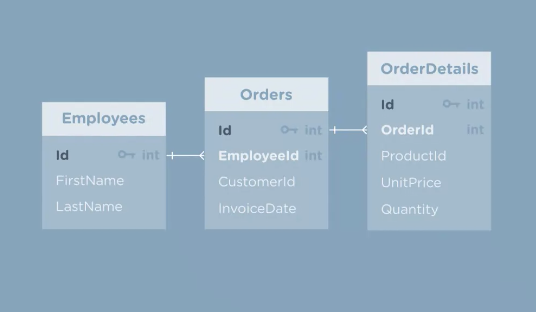
\includegraphics[width=\linewidth]{images/part_1_notes_1.png}
\end{center}

\begin{itemize}
    \item can only reference earlier WITH expression
    \item cannot reference latter WITH expressions

    \bigskip

    \underline{\textbf{Example:}}

    \bigskip

    \begin{lstlisting}[language=SQL]
    WITH
    all_sales AS (
        SELECT Orders.Id AS OrderId, Orders.EmployeeId,
        SUM(OrderDetails.UnitPrice * OrderDetails.Quantity) AS invoice_total
        FROM Orders
        JOIN OrderDetails ON Orders.id = OrderDetails.OrderId
        GROUP BY Orders.ID
    ),
    revenue_by_employee AS (
        SELECT EmployeeId, SUM(invoice_total) AS total_revenue
        FROM all_sales //<- From Earlier WITH
        GROUP BY EmployeeID
    ),
    sales_by_employee AS (
        SELECT EmployeeId, COUNT(*) AS sales_count
        FROM all_sales //<- From Earlier WITH
        GROUP BY EmployeeID
    )
    SELECT
    Employees.Id,
    Employees.LastName,
    revenue_by_employee.total_revenue,
    sales_by_employee.sales_count,
    revenue_by_employee.total_revenue/sales_by_employee.sales_count AS
                                                    avg_revenue_per_sale
    FROM revenue_by_employee
    JOIN sales_by_employee ON revenue_by_employee.EmployeeId = sales_by_employee.EmployeeId
    JOIN Employees ON revenue_by_employee.EmployeeId = Employees.Id
    ORDER BY total_revenue DESC
    \end{lstlisting}

\end{itemize}



\end{document}